\lecture{Operators and plots in Matlab}{14/10/2025}
\section{Conditional operators}
Gli operatori condizionali e i cicli sono costrutti fondamentali della programmazione che permettono di controllare il flusso di esecuzione di un programma.
Le istruzioni condizionali (\emph{if}, \emph{elseif}, \emph{else}) consentono di eseguire porzioni di codice solo se una certa condizione logica risulta vera.
I cicli, invece, permettono di ripetere un insieme di operazioni:
con \emph{for} le istruzioni vengono ripetute a seconda della condizione, mentre con \emph{while} la ripetizione continua finché la condizione resta verificata.
Questi strumenti rendono i programmi più flessibili, consentendo di gestire decisioni e iterazioni in modo dinamico.
Se si ha studiato qualche linguaggio di programmazione prima, come \emph{C}, \emph{Python},
\emph{Java}\dots si ha già un'ottima base, rivediamo comunque giusto la parte che differenzia i cicli e
gli operatori condizionali in Matlab rispetto ai linguaggi classici.
\subsection{If statement}
\begin{matlab}
a = 109;

if(a == 0 )
    fprintf('a = \%d\n', a);
elseif(a > 0)
    fprintf('a > 0 perche` a = \%d\n', a);
else
    fprintf('a < 0 perche` a = \%d\n', a);
end
\end{matlab}
Come si può vedere esiste \verb|if|, \verb|elseif| ed \verb|else|.

Inoltre ogni statement deve terminare con \verb|end|.

\subsection{For and while}
\subsubsection{For cycle}
\begin{verbatim}
for(a:b:c)
    instructions;
end
\end{verbatim}

Il ciclo \verb|for| è formato da:
\begin{itemize}
    \item \verb|a|: corrisponde all'\emph{initial value}, la variabile da cui inizia il counter del ciclo;
    \item \verb|b|: corrisponde allo \emph{step}, ovvero l'incremento della variabile;
    \item \verb|c|: il valore di termine a cui deve arrivare \verb|a| per fermare il ciclo.
\end{itemize}
È differente dal ciclo for usato ad esempio in Java, ma ha lo stesso concetto alla base.

\bigskip
\begin{matlab}
a = 109
for a=0:2:10
    fprintf('Current value of a in loop: \%d\n', a);
end
\end{matlab}

\subsubsection{While cycle}
\begin{verbatim}
while(condition)
    instructions;
    (typically updating condition)
end
\end{verbatim}
Il ciclo while è come quelli dei linguaggi di programmazione classici, vi si inserisce un istruzione dentro e l'aggiornamento della variabile.
\begin{matlab}
a=0;
while(a<=10)
    fprintf('a e` \%d\n', a);
    a=a+1;
end
\end{matlab}

\begin{note}[Boolean operators]
Si può notare che, se definissi la variabile \verb|a| come \verb|a=true|, la variabile verrà registrata come \verb|a=1|, mentre verrà registrata come \verb|a=0| se definita come \verb|a=false|.
\end{note}

\section{Logical operators}
Gli operatori logici sono utilizzati per scrivere condizioni negli statement e nei cicli. Producono come output $ 0 $  se \emph{falso} o $ 1 $ se \emph{vero}.
\paragraph{AND} L'operatore ``AND'' (\&) restituisce \emph{true} solo se entrambe le condizioni sono vere.
\paragraph{OR} L'operatore ``OR'' ($ || $) restituisce \emph{true} se almeno una delle condizioni è vera.
\paragraph{Equal To} L'operatore ``Equal To'' ($ a==b $) restituisce \emph{true} se $ a $ è uguale a $ b $.
\paragraph{Different from} L'operatore ``Different from'' (\verb|a~=b|) restituisce \emph{true} se $ a $ è diverso da $ b $.
\paragraph{Greater than} L'operatore ``Greater than'' ($ a>b $) restituisce \emph{true} se $ a $ è maggiore di $ b $.
\paragraph{Greater than or equal to} L'operatore ``Greater than or equal to'' ($ a>=b $) restituisce \emph{true} se $ a $ è maggiore o guale di $ b $.
\begin{note}
Riguardo gli operatori $ > $ e $ >= $, troviamo la controparte $ < $ e $ <= $.
\end{note}
\newpage
\begin{example*}\end{example*}
\begin{matlab}
n=5;
    for i = 1:n
        if (i==1)||(i==3)
            a(i) = i;
        else
            a(i) = 2*i;
        end
    end
\end{matlab}
\begin{example*}\end{example*}
\begin{matlab}
% Esempio 1: Operazioni logiche di base
a = 5; b = 3;
ris1 = (a > 2) & (b < 4);   % true
ris2 = (a == 5) | (b == 5); % true
ris3 = ~(a < b);            % true

% Esempio 2: Operatori a corto circuito
if (a > 0) && (b > 0)
    disp('Entrambi positivi');
end
\end{matlab}


\section{Scripts and functions}
Come nei linguaggi di programmazione classici, anche su Matlab è possibile creare Script e Funzioni, in modo però un po' diverso dal tradizionale.

In Matlab, script e funzioni vengono salvati in file separati, ciascuno con il nome del file uguale a quello dello script o della funzione principale contenuta.
Ad esempio, una funzione chiamata \emph{somma} dovrà essere salvata nel file \emph{somma.m}.

Tali file possono essere eseguiti in diversi modi:
\begin{itemize}
    \item \textbf{Chiamata diretta} dalla \emph{Command Window}, digitando semplicemente il nome del file (senza estensione):
    \begin{verbatim}
    >> somma
    \end{verbatim}
    \begin{note}
    Questo caso funziona solo se la funzione non ha bisogno di parametri in input!
    \end{note}

    \item \textbf{Esecuzione tramite un altro script o funzione}, ovvero richiamandoli all'interno di un codice MATLAB:
    \begin{verbatim}
    risultato = somma(3, 5);
    \end{verbatim}
    \begin{note}
    Quando voglio richiamare in un file main una funzione contenuta in un altro file, quest'ultimo deve trovarsi:
    \begin{itemize}
        \item nella stessa directory del file main;
        \item in una cartella inclusa nel \emph{path} di Matlab.
    \end{itemize}
    \end{note}

    \item \textbf{Esecuzione manuale} tramite l'editor MATLAB, premendo il pulsante \emph{Run}.
\end{itemize}

È importante ricordare che:
\begin{itemize}
    \item Gli \emph{script} non accettano argomenti in ingresso né restituiscono valori in uscita.
    \item Le \emph{funzioni}, invece, possono ricevere parametri di input e restituire risultati di output.
\end{itemize}

\paragraph{Script}
Gli script sono semplicemente delle liste di comandi pronti all'uso.
\begin{matlab}
% file: calc.m
% Script che esegue operazioni mat.
x = 5;
y = 3;

somma = x + y;
prodotto = x * y;
media = (x + y) / 2;

disp('Risultati:')
disp(['Somma: ', num2str(somma)])
disp(['Prodotto: ', num2str(prodotto)])
disp(['Media: ', num2str(media)])
\end{matlab}
\begin{matlabconsole}
>> calc
Risultati:
Somma: 8
Prodotto: 15
Media: 4
\end{matlabconsole}

\paragraph{Functions}
Per creare una funzione si usa il seguente:
\begin{verbatim}
function [outputArg] = nameFuction(inputArg)
    %nameFuction docs
    Instructions
end
\end{verbatim}
Matlab usa una notazione particolare per la dichiarazione delle funzioni.
\begin{itemize}
    \item \verb|outputArg| sono gli argomenti che la funzione ritorna;
    \item \verb|inputArg| sono gli argomenti dati alla funzione in fase di chiamata.
\end{itemize}
\begin{note}
Utilizzando il comando \verb|help nameFuction| nella console di Matlab, verrà stampata la descrizione della funzione. Si può creare la descrizione tramite:
\begin{verbatim}
%nameFunction descrizione funzione
\end{verbatim}
inserito subito sotto la riga di dichiarazione della funzione.
\end{note}

\begin{matlab}
% file: areaRett.m
function [area]=areaRett(base,altezza)
    %areaRett(base,altezza) ritorna
    %l'area di un dato rettangolo
    area = base * altezza;
end
\end{matlab}
\begin{matlabconsole}
>> help areaRett
 areaRett(base,altezza) ritorna l'area di un dato rettangolo

 >> areaRett(10,5)
ans =
    50
\end{matlabconsole}

\subsection{Random generation}
In Matlab si possono generare valori in modo casuale.

\paragraph{rand()} Tramite la funzione \verb|rand()| si genera un numero casuale tra $ [0,1] $.
\subparagraph{rand(n,m)} Tramite la funzione \verb|rand(n,m)| si genera una matrice di numeri randomici tra $ [0,1] $.
\begin{matlab}
% Random generation function
rand()
rand(2,5)
\end{matlab}
\begin{matlabconsole}
>> random

ans =
0.9502

ans =
0.0344  0.3816  0.7952  0.4898  0.6463
0.4387  0.7655  0.1869  0.4456  0.7094
\end{matlabconsole}

\paragraph{randi(n)} La funzione \verb|randi(n)| genera un intero casuale contenuto tra $ \{1,\dots,n\} $.
\begin{matlab}
randi(50)
\end{matlab}
\begin{matlabconsole}
>> random
ans =
    28
\end{matlabconsole}

\paragraph{randn()} Genera numeri casuali distribuiti normalmente.

Questo vuol dire che genera un numero secondo una distribuzione gaussiana con media 0 e deviazione standard 1 ($ \mu = 0, \sigma = 1 $).

\subparagraph{randn(n,m)} Genera una matrice di grandezza $ n,m $ con numeri casuali distribuiti normalmente.

\begin{matlab}
randn(1)
randn(2,3)
\end{matlab}
\begin{matlabconsole}
>> random

ans =
   -1.0335

ans =
    1.2951   -0.4953   -0.6573
    2.7681    0.4688   -1.7170
\end{matlabconsole}

\begin{note}
Se scrivessi semplicemente \verb|randn(n)|, senza inserire il secondo numero $ m $, mi viene generata una matrice quadrata $ n \times n $.
\begin{matlab}
randn(2)
\end{matlab}
\begin{matlabconsole}
>> random

ans =
    1.9779    1.0374
    0.7953    2.3603
\end{matlabconsole}
\end{note}

Se volessi generale una distribuzione con media $ \mu $ e deviazione standard $ \sigma $ personale si può fare:
\[
  x = \mu + \sigma \cdot \text{randn($ n,m $)}
\]

\begin{matlab}
mu = 10;
sigma = 2;
x = mu + sigma * randn(3, 3)
\end{matlab}
\begin{matlabconsole}
>> random

x =
   10.2807    7.9100   12.8291
   10.4752   11.9315    8.1516
    8.6569    9.5605    8.8117
\end{matlabconsole}

Un evento che accade con probabilità $ p $ può essere simulato tramite:
\begin{verbatim}
if rand<p
    instructions;
end
\end{verbatim}

\begin{example}\end{example}
\begin{matlab}
p=0.8;
x=rand();
if x<p
    disp('Dentro lo statement')
    disp(p);
end
disp(x);
\end{matlab}
\begin{matlabconsole}
>> random
Dentro lo statement
    0.8000

    0.6557

>> random
    0.8583
\end{matlabconsole}
Nel primo run dello script abbiamo $ x=0.6557 $ e $ p=0.8000 $, quindi si entra nell'if.

Nel secondo run abbiamo $ x=0.8583 $, quindi abbiamo $ x>p $ che rende la condizione dell'if \emph{falsa}.

\section{Figures and plots} \label{sec:plots}
Se vogliamo entrare nell'ambiente ``figure'', basta digitare all'inzio del file \verb|figure|.
\begin{note}
Ricordiamo che è meglio creare un file a parte per ogni questione, in questo caso lavoriamo sul file \verb|figures.m|.
\end{note}

\subsection{Plotting a function}
Se vogliamo disegnare un grafico cartesiamo, lo facciamo tramite il comando \verb|plot(x,y)|.

Di seguito vediamo un esempio, poi chiariamo vari comandi e funzioni.
\begin{example}\end{example}
\begin{matlab}
% Grafico della funzione f(x) = x^2
x = -5:0.1:5;     % intervallo di x
y = x.^2;         % ATTENZIONE: potenza elemento  per elemento (.^)

figure
plot(x, y, 'LineWidth', 2)
grid on

xlabel('x')
ylabel('f(x)')
title('f(x) = x^2')

% Linee di bellezza
xline(0, '--k');
yline(0, '--k');
print('les_02-01', '-depsc') % Print img
\end{matlab}
Innanzitutto, cominciamo col dichiarare:
\begin{itemize}
    \item $ x $ come vettore riga con punti equidistanti da uno \emph{step}. In questo caso facciamo: $ x=-5:0.1:5 $;
    \item $ y $ come la funzione che vogliamo rappresentare, in questo caso avremo $ y=x^{2} $.
\end{itemize}

Poi dichiaramo l'inizio dell'ambiente \emph{figure}, questo ci servirà più avanti per manipolare certe figure e
``plottarci'' sopra. Ad esempio, si potrebbe assegnare una figura ad una variabile tramite \verb|a=figure(1)|, ma questo lo vedremo poi più avanti.

Utilizzimo la funzione \verb|plot()| per iniziare a disegnare la funzione, ad esso viene passato:
\begin{itemize}
    \item $ x $, il vettore riga $ -5:0.1:5 $;
    \item $ y $, la funzione $ x^{2} $;
    \item `\verb|linewidth|', che cambia lo spessore delle linee;
    \item $ 2 $, il nuovo spessore delle linee, il valore di default sarebbe $ 1 $.
\end{itemize}

Tramite \verb|grid on| attiviamo la griglia quadrata in background della funzione e tramite i comandi
\verb|xlabel()| e \verb|ylabel()| si possono cambiare i nomi delle etichette a bordo del grafico.

Tramite \verb|title('')| si assegna un titolo al grafico, tramite \verb|xline()| ed \verb|yline()| vengono
aggiunte delle linee nel grafico, in questo caso fatte per rendere il tutto più leggibile.
Infine troviamo il comando \verb|print('les_02-01', '-depsc')|, che non fa altro che scaricare nella cartella root
l'immagine appena generata da Matlab in formato ``eps'', in modo che io possa utilizzarla su \LaTeX{}.
Possiamo finalmente vedere la funzione nella figura \ref{fig:les_02-01}.

\begin{figure}[h]
    \centering
    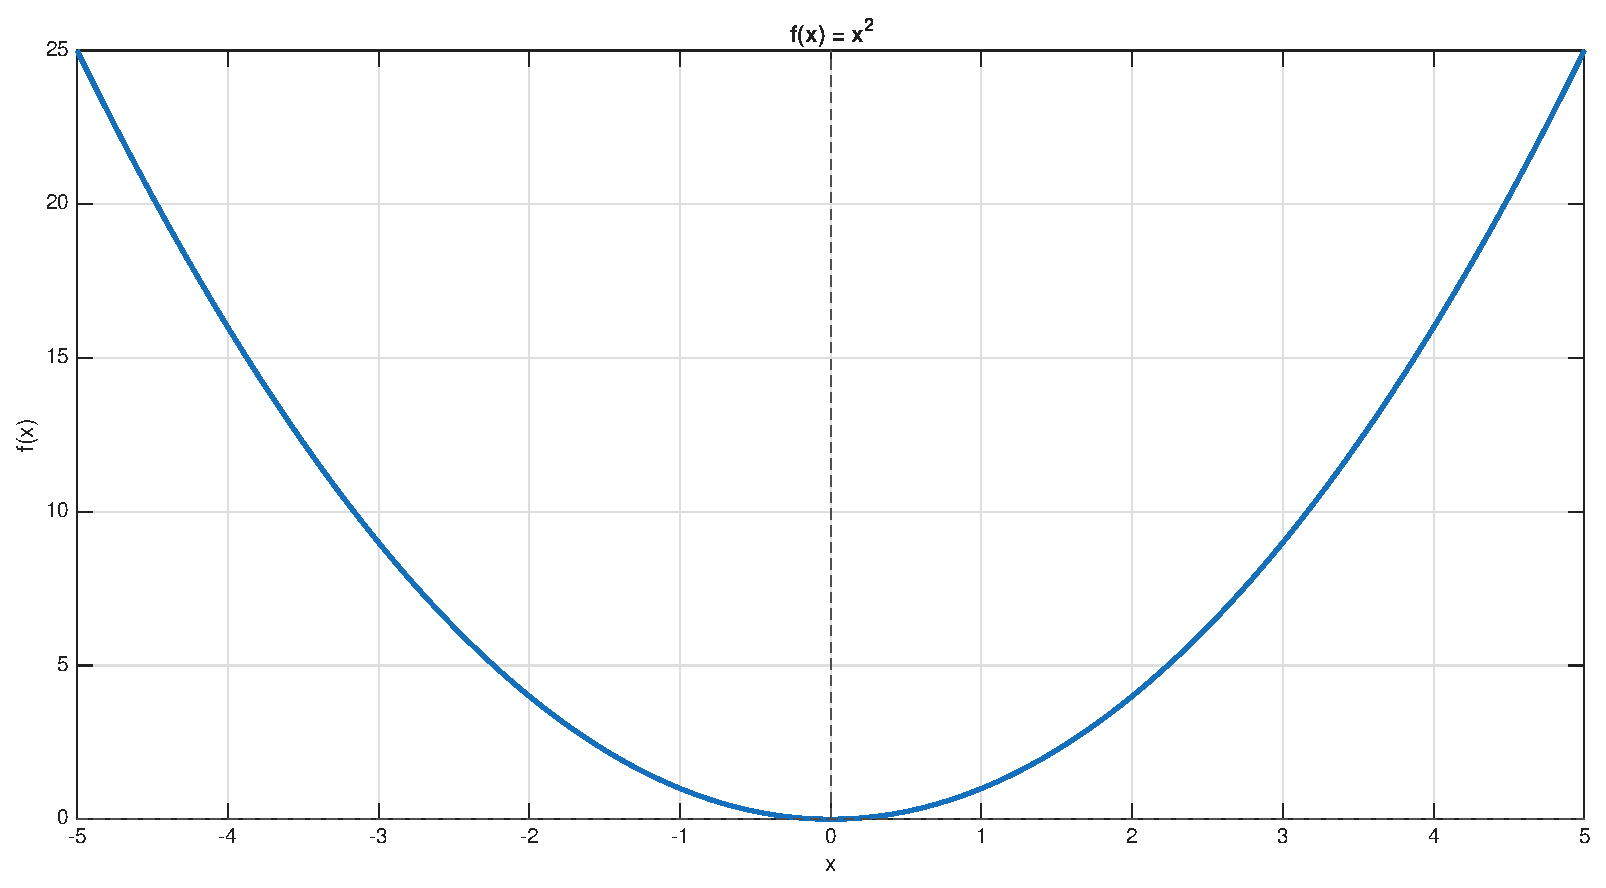
\includegraphics[width=\linewidth]{assets/les_02-01.eps}
    \caption{Plot della funzione $ f(x)=x^{2} $}
    \label{fig:les_02-01}
\end{figure}

\paragraph{sin(x) and cos(x) plotting}
Se volessimo produrre il grafico delle funzioni $ \sin(x) $ e $ \cos(x) $ sullo stesso grafico, potremmo
farlo tramite:
\begin{matlab}
a=figure(1)

x = 0:pi/100:2*pi;
y1 = sin(x);
y2 = cos(x);

plot(x,y1,x,y2);
grid on
\end{matlab}
Vediamo l'immagine \ref{fig:sinx-cosx} a riguardo.


\begin{figure}[h!]
    \centering
    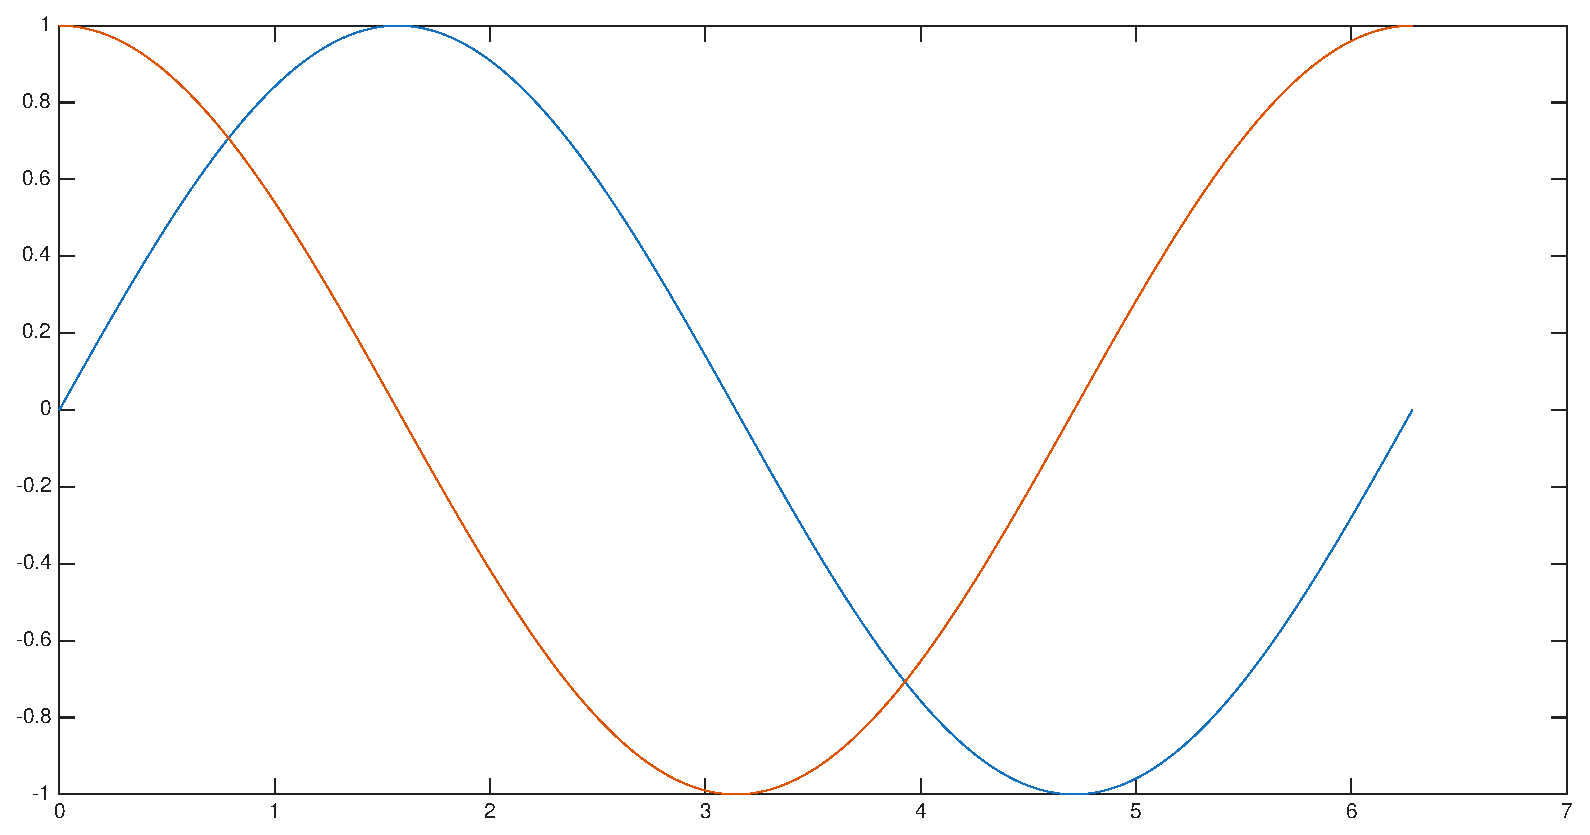
\includegraphics[width=\linewidth]{assets/les_02-figures.eps}
    \caption{Plot delle funzioni $ f(x)=\sin(x) $ e $ g(x)=\cos(x) $}
    \label{fig:sinx-cosx}
\end{figure}

\newpage
\begin{note}
Possiamo notare che sono un coglione e nella figura \ref{fig:sinx-cosx} manca l'opzione \verb|grid on| perché ho selezionato il file prima della modifica.
\end{note}

\subsubsection{More commands and methods for plots}
Vediamo altri comandi e metodi per creare figure e funzioni su Matlab (praticamente l'essenza del linguaggio).
